\documentclass[fontset=windows]{ctexart}

\usepackage{graphicx}
\graphicspath{ {./images/} }

\title{Vim实用技巧}
\author{潘潘}

\begin{document}

\maketitle

\section{寄存器与宏}

Vim的寄存器是一组用于保存文本的简单容器。

寄存器的设计体现了Vim中对于“记录”和“取用”这两个概念的思考。寄存器提供了一组文本容器,可以存放完全由可见字符组成的一段文本,也可以存放其中夹杂着不可见字符的按键操作序列。在Vim的使用过程中,需要进行记录并在某些时候再次取出使用的场景,是寄存器和宏完美覆盖的场景。

从简单到复杂,寄存器的使用覆盖了文本的摘取/粘贴、按键操作的记录与播放。结合Vim已有的多次重复某次操作机制(数字+操作),有很多耗时且易错的操作可以简单分解为宏命令的播放,其中可以夹杂其他寄存器的内容获取。

\begin{itemize}
	\item 修改寄存器内容
	\begin{itemize}
		\item visual模式下复制选定文本到寄存器x:\texttt{"xy}
		\item 对于复制操作有专用的寄存器0,而无名寄存器的内容会缺省地被复制、删除、剪切操作影响。
		\item normal模式下,qx将会开始录制按键操作到x中,再按一次q结束录制。
	\end{itemize}
	\item 取用寄存器内容
	\begin{itemize}
		\item insert或ex模式下读取寄存器x的可见字符部分到光标处:$\^$\texttt{rx}
		\item normal模式下读取寄存器x的内容到光标前后:\texttt{"xP}或者\texttt{"xp}
		\item normal模式下播放寄存器x中的内容:\texttt{@x}
		\item ex模式下播放寄存器x中的内容:\texttt{<motion>normal @x}
		\item 以及一些内置约定:
			\begin{figure}[h]
			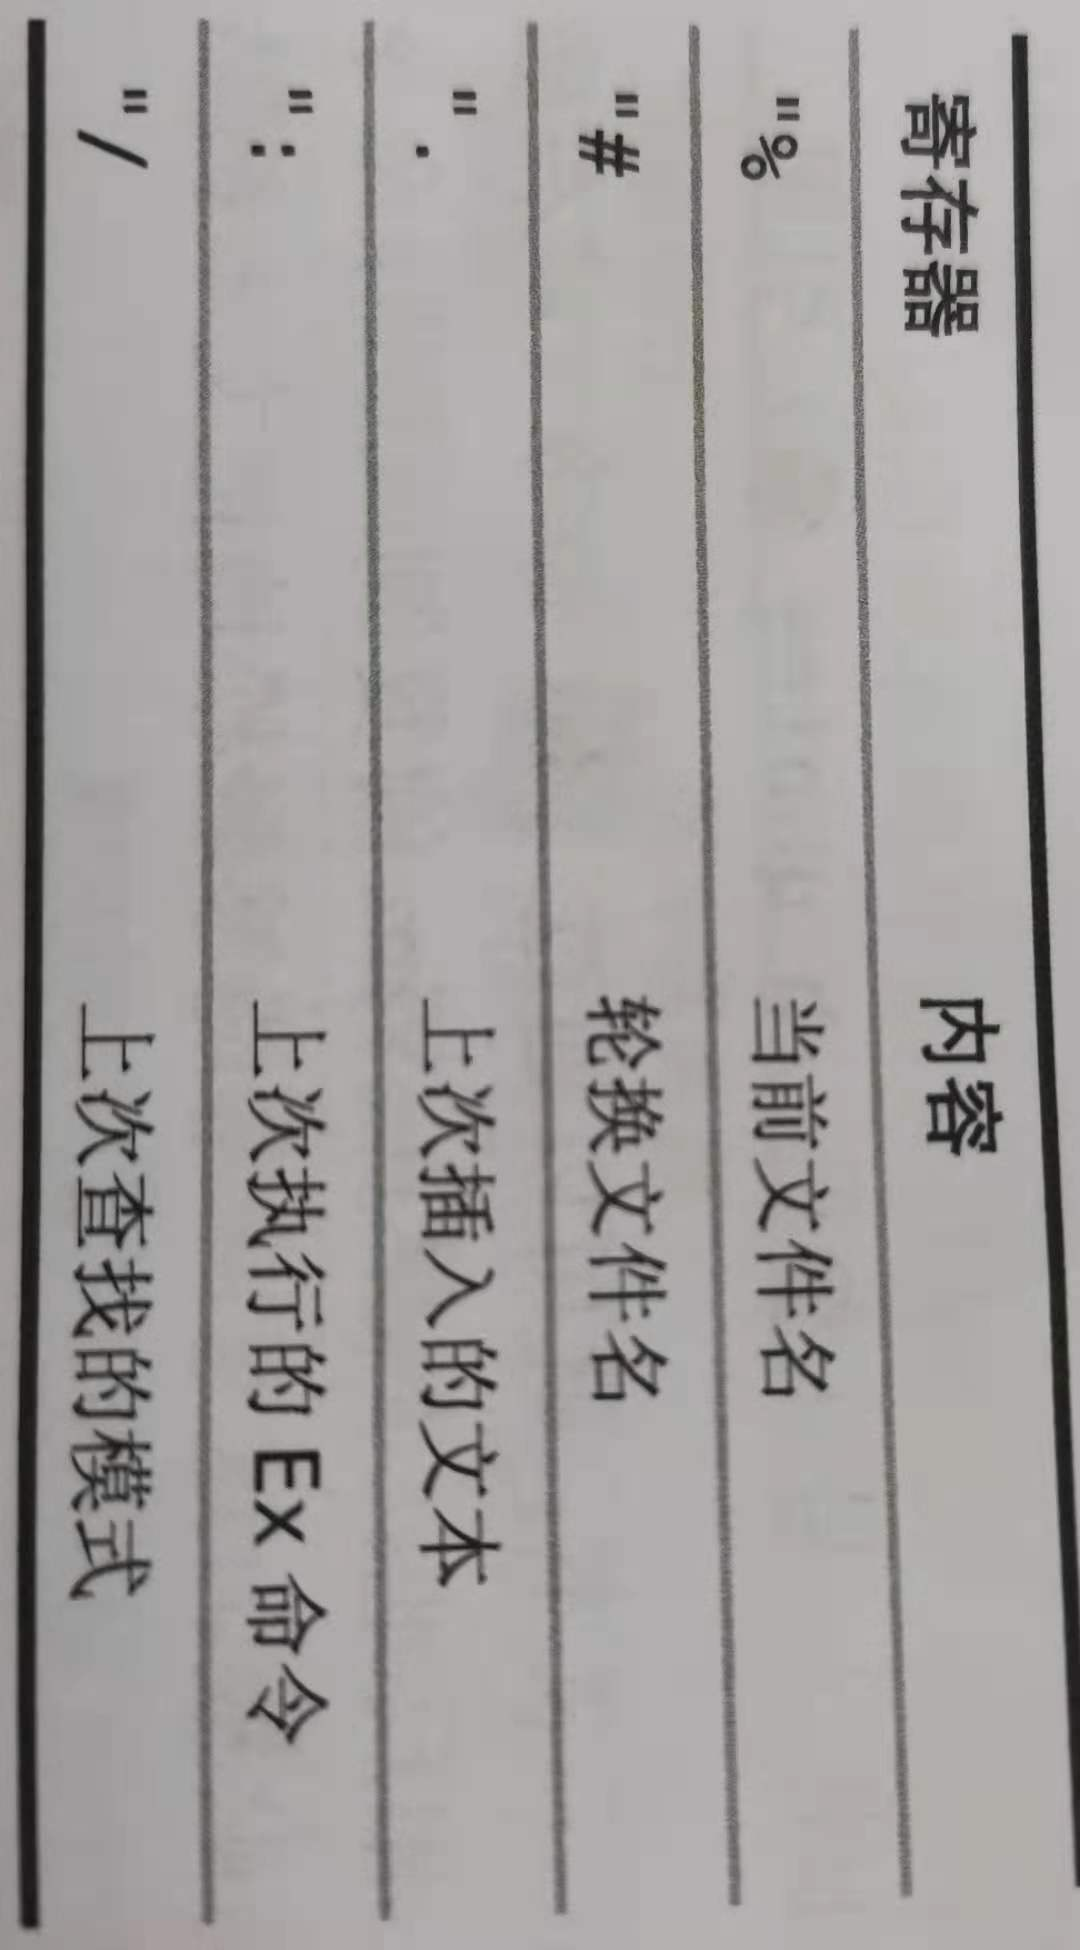
\includegraphics[width=0.5\textwidth, angle=90]{some_regs}
			\end{figure}
	\end{itemize}
\end{itemize}

\end{document}
